\documentclass[a4paper]{report}
\usepackage[utf8]{inputenc}
\usepackage[T1]{fontenc}
\usepackage{textcomp}

\usepackage{url}

\usepackage{hyperref}
\hypersetup{
    colorlinks,
    linkcolor={black},
    citecolor={black},
    urlcolor={blue!80!black}
}

\usepackage{graphicx}
\usepackage{wrapfig}
\usepackage{adjustbox}
\usepackage{float}
\usepackage[usenames,dvipsnames]{xcolor}

\usepackage{listings}

\lstset{
    language=Python,
    basicstyle=\ttfamily\footnotesize,
    keywordstyle=\color{blue},
    stringstyle=\color{red},
    commentstyle=\color{gray},
    showstringspaces=false,
    frame=single,
    numbers=left,
    numberstyle=\tiny,
    breaklines=true,
    tabsize=4
}

% \usepackage{cmbright}

\usepackage{amsmath, amsfonts, mathtools, amsthm, amssymb}
\usepackage{mathrsfs}
\usepackage{cancel}

\newcommand\N{\ensuremath{\mathbb{N}}}
\newcommand\R{\ensuremath{\mathbb{R}}}
\newcommand\Z{\ensuremath{\mathbb{Z}}}
\renewcommand\O{\ensuremath{\emptyset}}
\newcommand\Q{\ensuremath{\mathbb{Q}}}
\newcommand\C{\ensuremath{\mathbb{C}}}
\let\implies\Rightarrow
\let\impliedby\Leftarrow
\let\iff\Leftrightarrow
\let\epsilon\varepsilon

% horizontal rule
\newcommand\hr{
    \noindent\rule[0.5ex]{\linewidth}{0.5pt}
}

\usepackage{tikz}
% \usepackage{tikzmark}
\usepackage{pgfplots}
\usepackage{tikz-cd}

\usetikzlibrary{calc, arrows.meta, positioning, angles, quotes, patterns}

% theorems
\usepackage{thmtools}
\usepackage{thm-restate}
\usepackage[framemethod=TikZ]{mdframed}
\mdfsetup{skipabove=1em,skipbelow=0em, innertopmargin=12pt, innerbottommargin=8pt}

\theoremstyle{definition}

\makeatletter

\declaretheoremstyle[
    headfont=\bfseries\sffamily\color{ForestGreen!70!black}, bodyfont=\normalfont,
    mdframed={
        linewidth=2pt,
        rightline=false, topline=false, bottomline=false,
        linecolor=ForestGreen, backgroundcolor=ForestGreen!5,
    }
]{thmgreenbox}

\declaretheoremstyle[
    headfont=\bfseries\sffamily\color{NavyBlue!70!black}, bodyfont=\normalfont,
    mdframed={
        linewidth=2pt,
        rightline=false, topline=false, bottomline=false,
        linecolor=NavyBlue, backgroundcolor=NavyBlue!5,
    }
]{thmbluebox}

\declaretheoremstyle[
    headfont=\bfseries\sffamily\color{NavyBlue!70!black}, bodyfont=\normalfont,
    mdframed={
        linewidth=2pt,
        rightline=false, topline=false, bottomline=false,
        linecolor=NavyBlue
    }
]{thmblueline}

\declaretheoremstyle[
    headfont=\bfseries\sffamily\color{RawSienna!70!black}, bodyfont=\normalfont,
    mdframed={
        linewidth=2pt,
        rightline=false, topline=false, bottomline=false,
        linecolor=RawSienna, backgroundcolor=RawSienna!5,
    }
]{thmredbox}

\declaretheoremstyle[
    headfont=\bfseries\sffamily\color{RawSienna!70!black}, bodyfont=\normalfont,
    numbered=no,
    mdframed={
        linewidth=2pt,
        rightline=false, topline=false, bottomline=false,
        linecolor=RawSienna, backgroundcolor=RawSienna!1,
    },
    qed=\qedsymbol
]{thmproofbox}

\declaretheoremstyle[
    headfont=\bfseries\sffamily\color{NavyBlue!70!black}, bodyfont=\normalfont,
    numbered=no,
    mdframed={
        linewidth=2pt,
        rightline=false, topline=false, bottomline=false,
        linecolor=NavyBlue, backgroundcolor=NavyBlue!1,
    },
]{thmexplanationbox}

\declaretheorem[numberwithin=chapter, style=thmgreenbox, name=Definition]{definition}
\declaretheorem[sibling=definition, style=thmredbox, name=Corollary]{corollary}
\declaretheorem[sibling=definition, style=thmredbox, name=Proposition]{prop}
\declaretheorem[sibling=definition, style=thmredbox, name=Theorem]{theorem}
\declaretheorem[sibling=definition, style=thmredbox, name=Lemma]{lemma}
\declaretheorem[sibling=definition, style=thmbluebox,  name=Example]{eg}
\declaretheorem[sibling=definition, style=thmbluebox,  name=Nonexample]{noneg}
\declaretheorem[sibling=definition, style=thmblueline, name=Remark]{remark}




\declaretheorem[numbered=no, style=thmexplanationbox, name=Proof]{explanation}
\declaretheorem[numbered=no, style=thmproofbox, name=Proof]{preuve}
\declaretheorem[style=thmbluebox,  numbered=no, name=Exercise]{ex}
\declaretheorem[style=thmblueline, numbered=no, name=Note]{note}

% \renewenvironment{proof}[1][\proofname]{\begin{replacementproof}}{\end{replacementproof}}

% \AtEndEnvironment{eg}{\null\hfill$\diamond$}%

\newtheorem*{uovt}{UOVT}
\newtheorem*{notation}{Notation}
\newtheorem*{previouslyseen}{As previously seen}
\newtheorem*{problem}{Problem}
\newtheorem*{observe}{Observe}
\newtheorem*{property}{Property}
\newtheorem*{intuition}{Intuition}


\declaretheoremstyle[
    headfont=\bfseries\sffamily\color{RawSienna!70!black}, bodyfont=\normalfont,
    mdframed={
        linewidth=2pt,
        rightline=false, topline=false, bottomline=false,
        linecolor=RawSienna, backgroundcolor=RawSienna!5,
    }
]{todo}
\declaretheorem[numbered=no, style=todo, name=TODO]{TODO}


\usepackage{etoolbox}

\AtEndEnvironment{vb}{\null\hfill$\diamond$}%
\AtEndEnvironment{intermezzo}{\null\hfill$\diamond$}%




% http://tex.stackexchange.com/questions/22119/how-can-i-change-the-spacing-before-theorems-with-amsthm
% \def\thm@space@setup{%
%   \thm@preskip=\parskip \thm@postskip=0pt
% }

\usepackage{xifthen}

\def\testdateparts#1{\dateparts#1\relax}
\def\dateparts#1 #2 #3 #4 #5\relax{
    \marginpar{\small\textsf{\mbox{#1 #2 #3 #5}}}
}

\def\@lesson{}%
\newcommand{\lesson}[3]{
    \ifthenelse{\isempty{#3}}{%
        \def\@lesson{Lecture #1}%
    }{%
        \def\@lesson{Lecture #1: #3}%
    }%
    \subsection*{\@lesson}
    \testdateparts{#2}
}

% fancy headers
\usepackage{fancyhdr}
\pagestyle{fancy}

% \fancyhead[LE,RO]{Gilles Castel}
\fancyhead[RO,LE]{\@lesson}
\fancyhead[RE,LO]{}
\fancyfoot[LE,RO]{\thepage}
\fancyfoot[C]{\leftmark}
\renewcommand{\headrulewidth}{0pt}

\makeatother

% figure support (https://castel.dev/post/lecture-notes-2)
\usepackage{import}
\usepackage{xifthen}
\pdfminorversion=7
\usepackage{pdfpages}
\usepackage{transparent}
\usepackage[margin=0.8in]{geometry}
\newcommand{\incfig}[1]{%
    \def\svgwidth{\columnwidth}
    \import{./figures/}{#1.pdf_tex}
}

% %http://tex.stackexchange.com/questions/76273/multiple-pdfs-with-page-group-included-in-a-single-page-warning
\pdfsuppresswarningpagegroup=1
\pgfplotsset{compat=1.11}
\usepackage{subcaption}

\author{Yehor Korotenko}

\newcommand{\scalar}[2]{\langle #1, #2 \rangle}
\newcommand{\scalair}[1]{\left\langle #1 \right\rangle}

% fancy chapters
\usepackage{lipsum}
\usepackage[Lenny]{fncychap}
\ChNameUpperCase
\ChNumVar{\fontsize{40}{42}\usefont{OT1}{ptm}{m}{n}\selectfont}
\ChTitleVar{\Large\sc}



\title{Notes du cours d'Analyse et Géometrie}
\begin{document}
\maketitle
\tableofcontents

\begin{abstract}
Professeur: Christian Gérard
\begin{itemize}
    \item CC: 0.15\\
        Pour les CC une semaine avant CC le prof va envoyer une liste des question. Les CC durent 30 minutes en TD en semaines:
        \begin{itemize}
            \item 17/2
            \item 17/3
            \item 17/4
        \end{itemize}
    \item P: 0.35
    \item E: 0.5
\end{itemize}
Il y aura des démonstrations en examens
\end{abstract}


\chapter{Premier cours}
\section{Éspaces $\R^d$  $\C^d$}
\begin{definition}
    \[
        \R^d = \{ X = (x_1, \ldots, x_d), x_i \in \R\}
    \] 
    $x_1, \ldots, x_d$ coordonnées cartésiennes de X
\end{definition}
\begin{eg}
   $d = 2$ coordonnées polaires:  
   \begin{align*}
      &x = r \cos \theta \\
        & y = r \sin \theta\\
        &0 \le r \le  \infty \quad \theta \in [0, 2\pi[
   \end{align*}
   \begin{center}
       
\begin{tikzpicture}
    % Create the axis
    \begin{axis}[
        axis lines=middle,
        xmin=-1, xmax=3,
        ymin=-1, ymax=3,
        xlabel={$x$},
        ylabel={$y$},
        axis equal,
        height=6cm
    ]
        % Draw the vector
        \addplot[->, thick, blue] coordinates {(0,0) (3,2)} node[right] {$\vec{v}$};

        % Draw x-axis projection manually
        \draw[thick] (axis cs: 0,0) -- (axis cs: 3,0);

        % Use TikZ outside \addplot for \pic
        \node (A) at (2, 0) {};
        \node (C) at ($(0,0)!0.5!(3,2)$) {};
        \node (B) at (0, 0) {};
        \node[above] (_) at ($(0,0)!0.5!(3,2)$) {$r$};
        
        \pic [draw,-, black, angle eccentricity=1.2, angle radius=1cm,"$\theta$"] {angle = A--B--C};
    \end{axis}
\end{tikzpicture}
\end{center}
\end{eg}

\begin{definition}
    $\R^d$ est un espace vectoriel sur  $\R$ 
    \begin{align*}
        &\vec{X} + \vec{Y} = (x_1 + y_1, \ldots, x_d + y_d)\\
        &\lambda X = (\lambda x_1, \ldots, \lambda x_d) \quad \lambda \in \R\\
        &\vec{0}_d = \vec{0} = (0, \ldots, 0)
    \end{align*}
\end{definition}
\begin{definition}\label{def:prod_scalaire}
    Un \textbf{produit scalaire}:
    \[
    X \cdot Y = x_1y_1 + x_2y_2 + \ldots x_dy_d = \|X\|\|Y\|\cos(\theta) \text{ (où } \theta \text{ est une angle entre } X \text{ et } Y \text{)}
    \] 
\end{definition}
\begin{intuition}
    Ce produit nous dit \textit{how closely the vectors point in the same direction} (cosinus tend vers 1 quand $\theta$ tend vers 0º, et cosinus tend vers 0 quand  $\theta$ tend vers 90º). Et ce produit nous permet d'avoir une projection de $X$ sur $Y$ par la formule:
    \[
    Proj(X) = \frac{X \cdot Y}{\|Y\|} \cdot \frac{Y}{\|Y\|}
    \] 
    $X \cdot Y$ donne la longeur de  $X$ et  $Y$ ensemble, en divisant cette longeur par  $\|Y\|$ (la longeur de $Y$) on obtient la longeur de $X$ sur Y, il nous reste de multiplier cette longeur par un vecteur unitaire(de longeur 1) qui pointe dans la même direction que  $Y$, (on l'obtient par $\frac{Y}{\|Y\|}$)
   \begin{center}
      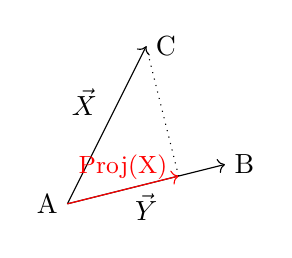
\begin{tikzpicture}
         \coordinate (A) at (0, 0); 
         \coordinate (B) at (2, 0.5);
         \coordinate (C) at (1, 2);
         \coordinate (newB) at (1.4117647059, 0.3529411765);
         \coordinate (dotBC) at (2, 1);
         \node[left] (_) at (A){A};
         \node[right] (_) at (B){B};
         \node[right] (_) at (C){C};
         \draw[->] (A) -- (B);
         \node[above left] (...) at ($(A)!0.5!(C)$) {$\vec{X}$};
         \node[below] (...) at ($(A)!0.5!(B)$) {$\vec{Y}$};
         \draw[->] (A) -- (C);
         \draw[->, red, thin] (A) -- (newB);
         \draw[dotted] (C) -- (newB);
         \node[above, red] (_) at ($(A)!0.5!(newB)$){\small Proj(X)};
      \end{tikzpicture} 
   \end{center}
\end{intuition}
\begin{prop}
    Produit scalaire respectes ces propriétés:
    \begin{enumerate}
        \item bilinaiarité $\quad \lambda \in \R$
            \begin{enumerate}
                \item $(X + Y) \cdot Z = X \cdot Z + Y \cdot Z$
                \item $(\lambda X) \cdot Z = \lambda (X \cdot Z)$
                \item $Z \cdot (X + Y) = Z \cdot X + Z \cdot Y$ 
                \item $Z \cdot (\lambda X) = \lambda (Z \cdot X)$
            \end{enumerate}
        \item symétrie $X \cdot Y = Y \cdot X$
        \item défini positif:  $X \cdot X \ge 0$ et $X \cdot X = 0 \iff X = 0_d$
    \end{enumerate}
\end{prop}
\begin{prop}
    \underline{Cauchy-Schwarz}:\\ 
    \[
        |X \cdot Y| \le (X \cdot X)^{\frac{1}{2}}(Y \cdot Y)^{\frac{1}{2}}
    \] 
\end{prop}
\begin{definition}\label{def:norm_eucl}
    La \textbf{norme euclidienne} d'un vecteur $X$ est noté:
   \[
       \|X\| = \left(\sum_{n=1}^{d} x_i^2\right)^{\frac{1}{2}} = \sqrt{x_1^2 + \ldots + x_d^2} = (X \cdot X)^{\frac{1}{2}}
   \] 
   souvent noté $\|X\|_2$
\end{definition}
\begin{intuition}
   Par le théorème de Pythogore, c'est une longeur de ce vecteur. 
\end{intuition}
\begin{prop}
    La norme suit ces propriétés:
   \begin{enumerate}
       \item $\|\lambda X\| = |\lambda|\|X\| \, X \in \R^d, \, \lambda \in \R$
       \item $\|X + Y\| \le \|X\| + \|Y\| \text{ (inégalité triangulaire)}$
       \item $\|X\| \ge 0$ et $\|X\| = 0 \iff X = 0_d$
   \end{enumerate}
\end{prop}
\begin{explanation}
    de (2)
    \begin{align*}
        \|X + Y\|^2 &= (X + Y)\cdot(X + Y) = X \cdot (X + Y) + Y \cdot (X + Y) = X \cdot X + X \cdot Y + Y \cdot X + Y \cdot Y\\
                    &= \|X\|^2 + 2X \cdot Y + \|Y\|^2 \le \|X\|^2 + 2\|X\| \|Y\| + \|Y\|^2 = (\|X\| + \|Y\|)^2
    \end{align*}
\end{explanation}
\begin{definition}
    Une \underline{norme} sur $\R^d$ est une application  $N: \: \R^d \to \R$ tell que:
    \begin{enumerate}
        \item $N(\lambda X) = |\lambda|N(X)$
        \item  $N(X + Y) \le N(X) + N(Y)$
        \item $N(X) \ge 0$ et $N(X) = 0 \iff X = 0_d$
    \end{enumerate}
\end{definition}
\begin{eg}
   \begin{align*}
       &\|X\|_1 = \sum_{n=1}^{d} |x_i|\\
       &\|X\|_{\infty} = \underset{1\le i \le n}{max} |x_i|
   \end{align*} 
\end{eg}
\section{Éspace $\C^d$}
\begin{definition}
    \[
        \C^d = \{ X = (x_1, \ldots, x_d): \: x_i \in \C\}
    \] 
    \begin{align*}
    &z \in \C \quad \overline{z} = a - ib \quad \overline{z}z = a^2 + b^2 \quad |z| = \sqrt{\overline{z}z} = \sqrt{a^2 + b^2}  \\
    &z = a + ib \qquad a = Re\,z,\,b = Im\,z\\
    &Re\,X = (Re\,x_1, \ldots, Re\,x_d) \in \R^d\\
    &Im\,X = (Im\,x_1, \ldots, Im\,x_d) \in \R^d\\
    &\underset{\in \C^d}{X} = \underset{\in \R^d}{Re\,X} + i\underset{\in \R^d}{\:Im\,X}\\
    \end{align*}
    $\C^d$ est un espace vécrotiel sur  $\C$ (même formules avec $\lambda \in \C$ corps des scalaires)
\end{definition}
\begin{definition}
    \underline{Produit scalaire:}
    \[
        (X|Y) = \sum_{n=1}^{d} \overline{x_i}y_i \in \C
    \] 
\end{definition}
\begin{prop}
   . 
   \begin{enumerate}
       \item $(X|Y)$ est "linéaire par rapport à Y"
           \begin{itemize}
               \item $(Z|X + Y) = (Z|X) + (Z|Y)$
               \item $(Z|\lambda X) = \lambda(Z|X) \quad \lambda \in \C$
               \item  $(Z|\lambda X + \mu Y) = \lambda(Z|X) + \mu(Z|Y)$
               \item  $(X + Y|Z) = (X|Z) + (Y|Z)$
               \item $(\lambda X|Z) = \overline{\lambda}(X|Z) \quad \lambda \in \C$
               \item $(\lambda X + \mu Y|Z) = \overline{\lambda}(X|Z) + \mu(Y|Z)$
           \end{itemize}
       \item $(Y|X) = \overline{(X|Y)}$
       \item $(X|X) = \sum_{n=1}^{d} \overline{x_i}x_i = \sum_{n=1}^{d} |x_i|^2$\\
           $(X|X) \ge 0$ et $(X|X) = 0 \iff X = 0_d$
   \end{enumerate}
\end{prop}
\begin{explanation}
    On a Cauchy-Schwarz:
    \begin{align*}
        (X|Y) \le (X|X)^{\frac{1}{2}}(Y|Y)^{\frac{1}{2}}
    \end{align*}
    même preuve qu'avant
\end{explanation}
On pose:
\begin{align*}
    \|X\| & \text{(ou }\|X\|_2\text{)}\\
          &= (X|X)^{\frac{1}{2}} = \left( \sum_{n=1}^{d} |x_i|^2 \right)^2
\end{align*}
norme hibertienne
\[
    \underset{\in \C^d}{\|X\|^2} = \underset{\in \R^d}{\|Re\,X\|^2} + i\underset{\in \R^d}{\:\|Im\,X\|^2}\\
\] 
\begin{lemma}
   \begin{align*}
       \|X\| = \underset{\|Y\|\le 1}{sup|(X|Y)|}
   \end{align*} 
\end{lemma}
\begin{explanation}
    $|(X|Y)| \le \|X\|\|Y\| \le \|X\|$ si $\|Y\| \le 1$
    \[
    \underset{\|Y\|\le 1}{sup|(X|Y)|}
    \] 
    \underline{Autre sens:} 
    \begin{align*}
        &X \neq 0 \quad Y =  \frac{X}{\|X\|} = \lambda X \quad \lambda = \frac{1}{\|X\|}\\
        &\|Y\| = |\lambda|\|X\| = \frac{1}{\|X\|}\|X\| = 1\\
        &(X|Y) = (X|\frac{X}{\|X\|}) = \frac{1}{\|X\|}(X|X) = \|X\|\\
        &sup \{|(X|Y)|: \, \|Y\| \le  1\}\\
        &\|X\| \le sup \{|(X|Y)|: \, \|Y\|\le 1\} \quad \text{(prendre }Y = \frac{X}{\|X\|}\text{)}
    \end{align*}

\end{explanation}
\underline{Autres normes sur $\C^d$}
\begin{itemize}
    \item $\|X\|_1 = \sum_{n=1}^{d} |x_i| \quad X \in \C^d$
    \item $\|X\|_{\infty} = \underset{1\le i \le d}{sup} |x_i|$
\end{itemize}
\section{Distance sur $\R^d$}
On oublie norme et produit scalaire. On introduit la distance
\begin{definition}\label{def:distance} La distance
    \[
        d(X, Y) = \|X - Y\| 
    \] 
\end{definition}
\begin{definition} La distance euclidienne
    \[
        d(X, Y) = \|X - Y\| = \sqrt{\sum_{n=1}^{d} (x_i - y_i)^2} 
    \] 
\end{definition}
\begin{prop}
    \begin{align*}
        d: \R^d &\longrightarrow \R \\
        (X, Y) &\longmapsto d((X, Y)) 
    .\end{align*}
    \begin{enumerate}
        \item $d(X, Y) = d(Y, X)$ (symétrie)
        \item $d(X, Y) \le d(X, Z) + d(Z, Y)$ (inég. triangulaire) $\forall X, Y, Z$ 
        \item $d(X, Y) \ge 0 \quad \forall X, Y$ et $d(X, Y) = 0 \iff X = Y$ 
    \end{enumerate}
\end{prop}
\begin{eg} Distances
   \begin{enumerate}
       \item $d_2(X, Y) = \|X - Y\|_2$ (distance euclidienne sur $\R^d$)
       \item $d_1(X, Y) = \|X - Y\|_1$\\
           $d_{\infty}(X, Y) = \|X - Y\|_{\infty}$
       \item distance logarithmique sur $\R_+$:  $d(a, b) = |b - a|$
           \[
               \log_{10}(a) = \frac{\log(a)}{\log(10)}
           \] 
           $x, y \in ]0, +\infty[$\\ 
           $d_{\log}(x, y) = |\log_{10}(\frac{y}{x})|$ \\
           $i$ est une distance sur  $]0, +\infty[$\\
           $d_{\log}(100, 110) = \log_{10}(1,1)$
       \item distance SNCF
           \begin{center}
               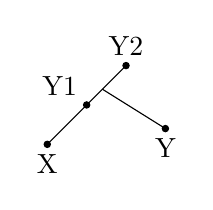
\begin{tikzpicture}
                  \coordinate (X) at (0, 0); 
                  \coordinate (Y) at (1.5, 0.2);
                  \coordinate (Y2) at (1, 1);
                  \coordinate (Y1) at ($(X)!0.5!(Y2)$);
                  \draw (X)--(Y2);
                  \draw (Y)--($(X)!0.7!(Y2)$);
                  \draw[fill=black] (X) circle (0.4mm);
                  \draw[fill=black] (Y) circle (0.4mm);
                  \draw[fill=black] (Y2) circle (0.4mm);
                  \draw[fill=black] (Y1) circle (0.4mm);
                  \node[below] (_) at (X){X};
                  \node[below] (_) at (Y){Y};
                  \node[above left] (_) at (Y1){Y1};
                  \node[above] (_) at (Y2){Y2};
               \end{tikzpicture}
               
           \end{center}
           $d(X, Y)$ distance usuelle dans  $\R^2$
           on pose:
            \begin{align*}
               \delta(X, Y) = \begin{cases}
                   d(X, Y) \text{ si } X, 0, Y \text{ alignés}\\
                   d(X, 0) + d(0, Y) \text{ sinon }
               \end{cases}
           \end{align*}
   \end{enumerate}
\end{eg}
\chapter{Éspaces métriques}
\begin{definition}
    $E$ muni d'une application de distance $d$ (voir Definition \ref{def:distance}) se note  $(E, d)$: \underline{espace métrique}
\end{definition}
\begin{remark}
   si $d_1 \neq d_2$ $(E, d_1)$ n'a rien à faire avec  $(E, d_2)$ 
\end{remark}
\begin{remark}
    Retenir la version suivante de l'inégalité triangulaire:
    \[
        |d(x, z) - d(y, z)| \le d(x, y)
    \] 
\end{remark}
\begin{remark}
    \underline{Distance induite:}\\
    Si $(E, d)$ espace métrique et  $U \subset E$. Je peux restreidnre $d$ à  $U \times U$:  $(U, d)$ est aussi un éspace metrique.
\end{remark}
\section{Boules dans un espace métrique}
\begin{definition}
    $(E, d)$ espace métrique. Soit  $x_0 \in E$ et $r \ge  0$
    \begin{enumerate}
        \item $B(x_0, r) = \{ x \in E: d(x_0, x) < r$ \} boule ouverte de centre $x_0$, de rayon $r$
        \item $B_f(x_0, r) = \{ x \in E: d(x_0, x) \le  r$\} boule fermée de centre $x_0$, de rayon $r$
    \end{enumerate}
\end{definition}
\begin{figure}
    \centering
    \begin{subfigure}{0.45\textwidth}
        \centering
        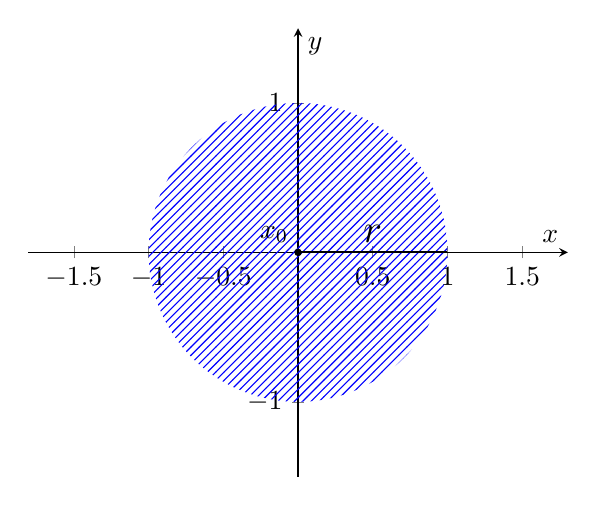
\begin{tikzpicture}
            \begin{axis}[
                axis equal, % Ensures the circle appears round
                axis lines=middle,
                xlabel={$x$},
                ylabel={$y$},
                xmin=-1.5, xmax=1.5,
                ymin=-1.5, ymax=1.5
                ]
                % Plot a circle with radius 1
                \addplot [
                    domain=0:360,       % Angle range
                    samples=200,        % Smoothness
                    fill=none,          % No solid fill color
                    pattern=north east lines, % Hatch pattern
                    pattern color=blue,
                    draw=none           % No outline
                    ] ({cos(x)}, {sin(x)}); 
                \node[above left] (_) at (0, 0){$x_0$};
                \draw[fill=black] (0, 0) circle (0.4mm);
                \draw[thick] (0,0)--(1,0);
                \node[above] (r) at ($(0,0)!0.5!(1,0)$){\Large$r$};
            \end{axis}
        \end{tikzpicture}
        \caption{boules ouverte (i.e $d(x_0, x) < r$)}
    \end{subfigure}
    \hfill
    \centering
    \begin{subfigure}{0.45\textwidth}
        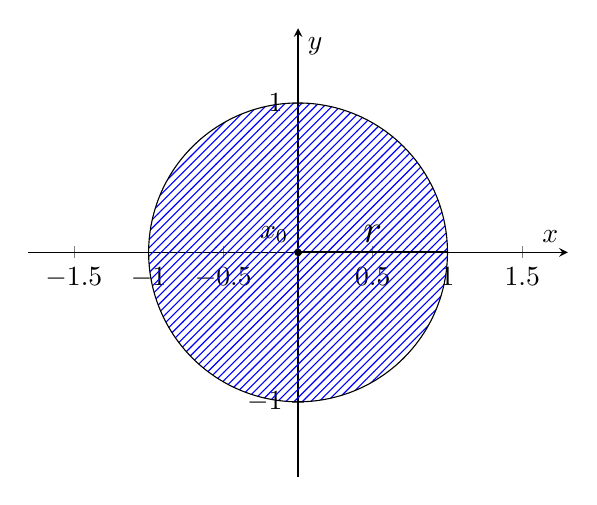
\begin{tikzpicture}
            \begin{axis}[
                axis equal, % Ensures the circle appears round
                axis lines=middle,
                xlabel={$x$},
                ylabel={$y$},
                xmin=-1.5, xmax=1.5,
                ymin=-1.5, ymax=1.5
                ]
                % Plot a circle with radius 1
                \addplot [
                    domain=0:360,       % Angle range
                    samples=200,        % Smoothness
                    fill=none,          % No solid fill color
                    pattern=north east lines, % Hatch pattern
                    pattern color=blue,
                    ] ({cos(x)}, {sin(x)}); 
                \node[above left] (_) at (0, 0){$x_0$};
                \draw[fill=black] (0, 0) circle (0.4mm);
                \draw[thick] (0,0)--(1,0);
                \node[above] (r) at ($(0,0)!0.5!(1,0)$){\Large$r$};
            \end{axis}
        \end{tikzpicture}
        \caption{boules fermée (i.e $d(x_0, x) \le r$)}
    \end{subfigure}
\end{figure}
\begin{lemma}.
   \begin{enumerate}
       \item $B(x_0, 0) = \O$ (car impossible d'avoir des points qui en distance sont strictement plus petit que 0)
       \item $B_f(x_0, 0) = \{x_0\}$
       \item $B(x_0, r_1) \subset B_f(x_0, r_1) \subset B(x_0, r_2)$ si $r_1 < r_2$
       \item $B(x_1, r_1) \subset B(x_0, r)$ si  $d(x_0, x_1) + r_1 \le r$
   \end{enumerate} 
   pic 5
\end{lemma}
\begin{explanation}
   Je suppose que $d(x_0, x_1) \le r$\\ 
   Soit $x \in B(x_1, r_1)$ donc $d(x_1, x) < r_1$ à montrer: $x \in B(x_0, r)$ (i.e $d(x_0, x) < r$?)\\
   L'inégalité triangulaire me dit:
   \begin{align*}
       d(x_0, x) &\le d(x_0, x_1) + d(x_1, x)\\
                 &< d(x_0, x_1) + r_1 \le r\\
                 &\implies x \in B(x_0, r)
   \end{align*}
\end{explanation}

\section{Parties bornées d'un éspace métrique}
\begin{definition}
    Une partie $A \subset E$ est bornée s'ils existent $x_0 \in E$ et  $r > 0$ tels que  $A \subset B(x_0, r)$
\end{definition}
\begin{prop}
    S'il existe $r > 0$ tel que $\forall x, y \in A, \, d(x, y) \le r$, alors $A$ est bornée.
\end{prop}
\begin{definition}
    La distance entre deux ensembles $A, B$ est:
     \[
         d(A, B) := \underset{x \in A, y \in B}{inf}d(x, y)
    \] 
    Intuitivement, on cherche deux points $x$ et  $y$ tel que la distance est la plus petite possible.
\end{definition}
\begin{definition}
    La distance entre un points $x$ et un ensemble  $B$ est:
     \[
         d(x, B) := \underset{y \in B}{inf}d(x, y)
    \] 
    La même intuition.
\end{definition}
\section{Topologie des éspaces métriques}
\begin{definition}
    .
    \begin{enumerate}
        \item Un ensemble $U \subset  E$ est \textbf{ouvert} si $\forall x \in U$ $\exists \delta > 0$ tel que $B(x, \delta) \subset U$.
        \item Un ensemble $F \subset E$ est \textbf{fermé} si $E \setminus F$ est ouvert, i.e $\forall x \in E \setminus F$ $\exists \delta > 0$ tel que $B(x, \delta) \subset E\setminus F$
    \end{enumerate}
\end{definition}
\begin{figure}[H]
    \centering
    \begin{subfigure}{0.45\textwidth}
        \centering 
        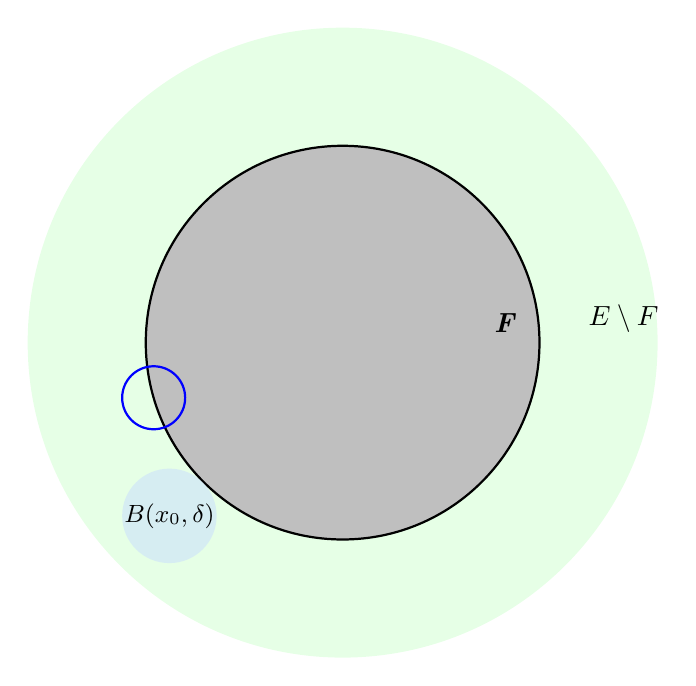
\begin{tikzpicture}
            % Define colors
            \definecolor{lightgreen}{RGB}{230, 255, 230}
            \definecolor{lightblue}{RGB}{200, 220, 255}
            \definecolor{darkgreen}{RGB}{0, 128, 0}

            % Large background circle
            \fill[lightgreen] (0, 0) circle (4cm);

            % Main circle
            \draw[thick, fill=lightgray] (0, 0) circle (2.5cm);
            \node[above right] at (1.8, 0) {\textbf{\textit{F}}};
            \node[above right] at (3, 0) {$E\setminus F$};

            % Small blue circle
            \draw[blue, thick] (-2.4, -.7) circle (0.4cm);

            % Highlighted area for excluded point
            \fill[lightblue, opacity=0.5] (-2.2, -2.2) circle (0.6cm);
            \node (_) at (-2.2, -2.2){\small $B(x_0, \delta)$};
        \end{tikzpicture}
        \caption{Un ensemble fermé\\
            \textit{À la borne, il est impossible de trouver une boules qui appartient à $F$, car il est impossible d'avoir une boule ouverte de  $r = 0$. Exemple: circle bleu foncé}\\
            \textit{Pour tout point dans $E \setminus F$ on peut trouver une boule ouverte}
        }
    \end{subfigure}
    \hfill
    \begin{subfigure}{0.45\textwidth}
        \centering
        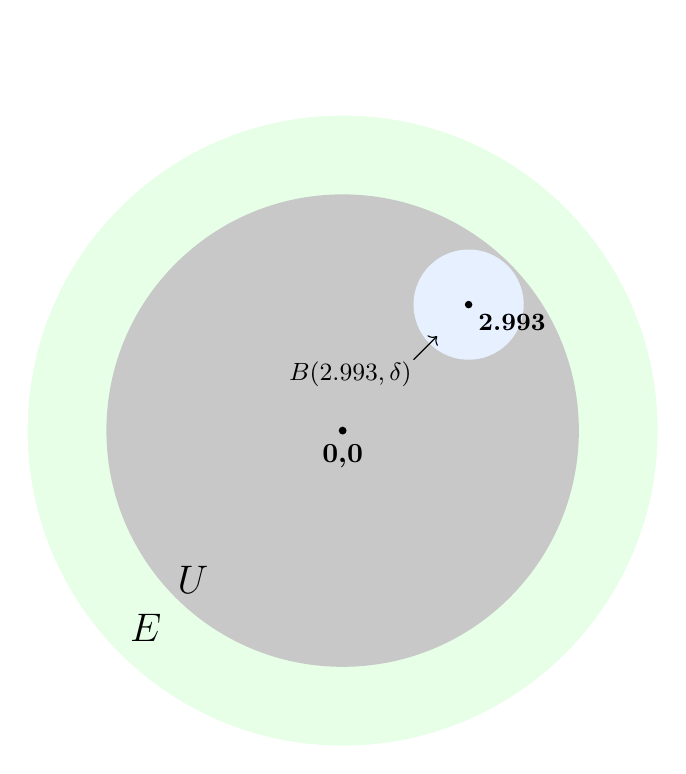
\begin{tikzpicture}
            % Define colors
            \definecolor{lightblue}{RGB}{230, 240, 255}
            \definecolor{lightgray}{RGB}{200, 200, 200}
            \definecolor{darkgreen}{RGB}{0, 128, 0}
            \definecolor{lightgreen}{RGB}{230, 255, 230}

            % Draw large circle
            \fill[lightgreen] (0, 0) circle (4cm);
            \fill[lightgray] (0, 0) circle (3cm);

            % Draw small circle
            \fill[lightblue] (1.6, 1.6) circle (0.7cm);
            \draw[fill=black] (1.6, 1.6) circle(0.4mm);
            \node[below right] at (1.6, 1.6) {\textbf{\small 2.993}};

            \draw[->] (0.9, 0.9)--(1.2, 1.2);
            \node[below left] (_) at (1, 1){\small $B(2.993, \delta)$};
            % Add points and labels
            \node[fill=black, circle, inner sep=1pt, label=below:{\textbf{0,0}}] at (0, 0) {};

            % Add text
            \node[right] at (1, 5) [align=left, text=darkgreen] {
                };
            \node (_) at (-1.9, -1.9){\Large $U$};
            \node (_) at (-2.5, -2.5){\Large $E$};
        \end{tikzpicture} 
        \caption{Un ensemble ouvert\\
            \textit{
                pour tout point pres de la borne
                on peut trouver une boule
                infiniment petite avec des
                points autour ce point inclu dans $U$.
            }
        }

    \end{subfigure}
    \caption{Démonstration des espaces ouverts et fermés}
\end{figure}

\begin{prop}.
    \begin{enumerate}
        \item 
            Une union des ensembles ouverts est aussi ouvert, idem avec l'intersection des ensembles ouverts. 
        \item  
            Une union des ensembles fermé est aussi fermé, idem avec l'intersection des ensembles fermé. 
    \end{enumerate}
\end{prop}

\section{Intérieur, adhérence, frontière}
Soit $A \subset E$. 
\begin{definition}
    Un point $x \in E$ est intérieur à $A$ s'il existe  $\delta > 0$ tel que  $B(x, \delta) \subset A$.\\
    Ensembles des points intérieur à $A$ se note  $Int(A)$ ou  $\mathring{A}$.
\end{definition}
\begin{intuition}
   $Int(A)$ est un ensemble qui est totalement dans  $A$ est se trouve loin des bords. 
\end{intuition}
\begin{tabular}[c]{@{}l@{}r@{}}
    \adjustbox{valign=t}{
    \parbox[t]{0.79\textwidth}{
    \begin{definition}
        Un point $x \in E$ est adhérent à  $A$ si  $\forall r > 0, \, B(x, r) \cap A \neq \O$ (toute boule centré dans $x$ intersecte  $A$).  \\
        Ensemble des points adhérents à $A$ se note  $Adh(A)$ ou  $\overline{A}$.
    \end{definition}
}
}
    &
    \hfill
    \adjustbox{valign=t}{
        \parbox[t]{0.2\textwidth}{
            \vspace{0.3cm}
    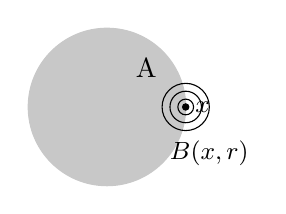
\begin{tikzpicture}
            \definecolor{lightgray}{RGB}{200, 200, 200}
        \filldraw[color=lightgray] (0,0) circle (1cm); 
        \coordinate (x) at (1, 0);
        \filldraw[color=black] (x) circle (0.4mm);
        \node[right] (_) at (x){\small $x$};
        \node (_) at (0.5, 0.5){A};

        \draw (x) circle (0.2cm);
        \draw (x) circle (0.3cm);
        \draw (x) circle (0.1cm);
        \node[below] (_) at (1.3, -0.3){\small $B(x, r)$};
    \end{tikzpicture} 
}
}
\end{tabular}
\begin{intuition}
   Si $A$ est ouvert (ses bords n'appartiennent pas à $A$), ses bords appartiennent à $Adh(A)$. Cette notion est utile pour completer des ensembles.
   \begin{eg}
       $\overline{\Q} = \R$ 
   \end{eg} 
\end{intuition}
\begin{definition}
    $Adh(A) \cap Adh(E \setminus A)$ est le bord de $A$ est s'appelle  la frontière de $A$.
\end{definition}
\section{Suite dans un éspace métrique}
\begin{definition}
    Une suite $(x_n)_{n \in \N}$ converge vers $x \in E$, si  $\forall \epsilon > 0, \exists N \in \N$ tel que :
    \[
    \forall n \ge N, \, d(x_n, x) \le  \epsilon
    \] 
\end{definition}
\begin{prop}
   Soit $A \in E$.\\ 
   \begin{enumerate}
       \item $x \in Adh(A)$ si et seulement si, il existe une suite $(x_n)_{n \in \N}$ d'éléments de $A$ telle que  $x_n \xrightarrow[n \to +\infty]{} x$ 
       \item $A$ est fermé (i.e contient sa frontière) si et seulement si la limite de toute suite  $(x_n)_{n \in \N}$ d'éléments de $A$ appartient à  $A$.
   \end{enumerate}
\end{prop}
\begin{intuition}
   \begin{enumerate}
       \item Si $(x_n)_{n \in \N}$ est d'éléments de  $A$ ($\forall n \in N, \, x_n \in A$), donc elle converge vers un éléments $x$ qui peut être soit dans  $A$, soit la borne des éléments de  $A$, alors à la frontière. 
       \item Si la limite de toute suite $(x_n)_{n \in \N}$ des éléments de  $A$ est aussi dans  $A$, alors la frontière de  $A$ est inclu dans  $A$. Car l'une des suites tend vers la borne.
   \end{enumerate} 
\end{intuition}
\begin{definition}
    Une suite $(x_n)_{x \in \N}$ est de Cauchy si  $\forall \epsilon > 0, \exists N \in \N$ tel que:
    \[
    \forall n, p \ge N, \, d(x_n, x_p) \le \epsilon
    \] 
\end{definition}
\begin{intuition}
   Une suite de Cauchy c'est comme on mesure un point et on le localise, i.e:
   \begin{enumerate}
       \item On dit qu'il est entre $0$ et  $1$.
       \item Ensuite, on precise plus et on dit qu'il est entre  $0.5$ et  $0.6$.
       \item Puis, entre  $0.55$ et  $0.56$
   \end{enumerate}
   On peut infiniment augmenter le niveau de précision. C'est ça l'idée d'une suite de Cauchy.
\end{intuition}
\begin{definition}
    Un éspace métrique $(E, d)$ est \textbf{complet} si toute suite  $(x_n)_{n \in \N}$ d'éléments de  $E$ converge vers une limite  $x$ qui appartient aussi à  $E$.
\end{definition}
\begin{eg}
    Un éspace métrique $(]0, 1], d)$ avec $d$ une distance euclidienne n'est pas complet, car  soit une suite: $x_n = \frac{1}{n}$ dont la limite est $0$. Par contre,  $0 \not\in ]0, 1]$. Donc cet éspace n'est pas complet. 
\end{eg}
\begin{figure}[h]
   \centering 
   \begin{tikzpicture}
       \draw[->] (-1, 0) -- (2, 0); 
       \node[below] (_) at (2,0){$x$};

       \node (_) at (0,0){]};
       \node[below] (_) at (0,-0.3){$0$};
       \node (_) at (1,0){]};
       \node[below] (_) at (1,-0.3){$1$};
       \draw[color=red] (0,0)--(1,0);
   \end{tikzpicture}
   \caption{$(]0, 1], d)$ n'est pas complet}
\end{figure}
\begin{eg}
   Un éspace $(\Q, d)$ n'est pas complet. Car on peut prendre une suite  $x_n$ tendant vers  $\sqrt{2} \not\in \Q$.
\end{eg}

\begin{figure}[H]
    \centering
    \incfig{q_not_complete}
    \caption{$\Q$ pas complet}
    \label{fig:q_not_complete}
\end{figure}

\begin{definition}
    Soit une suite $(x_n)_{n \in \N}$ et une application  $\phi:\N \to \N$ \underline{strictement croissante}. Une suite $(x_n)_{\phi(n)}$ est appellée une sous-suite.
\end{definition}
\begin{eg}
    Soit une application $\phi: \N \to \N$ telle que $\phi(n) = 2n$. Donc  $(x_n)_{\phi(n)}$ est une sous-suite de  $(x_n)_{n \in \N}$ et:
    \[
        (x_n)_{\phi(n)} = \{x_0, x_2, x_4, \ldots\}
    \] 
\end{eg}

\section{Compacité}
\begin{definition}
    Soit $F \subset E$. Un \textbf{recouvrement ouvert} de $F$, est une union des enesembles ouverts:  $\bigcup_{i \in I} U_i$ tel que $F \subset \bigcup_{i \in I} U_i$
\end{definition}
\begin{eg}
    Soit $F = ]0, 1[$. Soit $A = \left\{]\frac{1}{n}, 1 + \frac{1}{n}[, n \in N\right\}$. $F \subset \bigcup_{n \in N^{*}} A_n$ i.e union infinie des $A_i$ couvre $F$.
\end{eg}
\begin{definition}
    Un ensemble $F \subset E$ est \textbf{compact} si \underline{pour tout} recouvrement ouvert, i.e \underline{pour tout} union des ensembles ouvert $\bigcup_{i \in I} U_i$ qui couvre $F$, on peut prendre un nombre \underline{fini} des  $U_i$ et couvrir $F$.
\end{definition}
\begin{theorem}
    Un ensemble $K \subset E$ est compact, si toute suite $(x_n)_{n \in \N}$ des éléments de $K$, possede une sous-suite qui converge  vers un éléments $x \in K$.
\end{theorem}
\begin{intuition}
    S'il existe tel suite $(x_n)_{n \in \N}$ sans sous-suite convergente vers un éléments de  $K$, donc les valeurs sont en-dehors de  $K$ et donc il existe un ensemble qui couvre $K$  seulement avec un nombre infini des ensembles. 
\end{intuition}
Pourquoi a-t-on besoin de compacité? Car cela nous donne une
\begin{prop}
    Si $K \subset E$ est compact, alors $K$ est fermé et borné.\\
    Si $K$ est compact est  $F$ est borné, donc  $K \cap F$ est compact\\
    Si $K$ est compact, donc  $K$ est complet
\end{prop}
\begin{property}
    La différence entre \textit{compacité} et {complecité}:
    \begin{itemize}
        \item complecité nous assure qu'il n'y a pas de trou dans un espace
        \item compacité nous assure qu'un ensemble est fermé et borné
    \end{itemize}
\end{property}
\section{Limites et applications continues}
2


\end{document}

